\documentclass{article}
\usepackage[utf8]{inputenc}
\usepackage[T1]{fontenc}
\usepackage{graphicx}
\usepackage{caption}
\usepackage{subcaption}
\usepackage{graphicx}
\usepackage{amsmath, amsthm, amssymb}
\usepackage[backend=biber,style=numeric,natbib=true]{biblatex}
\usepackage[margin=2.8cm]{geometry} % set page margins
\usepackage{setspace}
\usepackage{parskip}
\usepackage{multirow}
\usepackage{array}
\usepackage{indentfirst}
\usepackage{booktabs}
\usepackage[bottom]{footmisc}
\usepackage{xcolor}
\usepackage[colorlinks=true, linkcolor=black]{hyperref}
\setlength{\footnotesep}{0.5cm} % set footnote seperation to 0.5cm
\setlength{\parindent}{1cm} \setstretch{1.15} \addbibresource{references.bib}% set paragraph indentation to 1cm

\newcommand{\titlefont}{\fontsize{21}{32}\selectfont}
\newcommand{\authorfont}{\fontsize{20.74}{24}\selectfont}
\begin{document}

\begin{titlepage}
  \centering
  \vspace*{5cm}
  {\titlefont\textbf{\color{black}Topic 3: Modelling of Real-life MIP Problems}\par}
  \vspace{1.5cm}
  {\authorfont\color{black} The Ikunbelievable Group\par}
  \vfill
\end{titlepage}

\tableofcontents
\clearpage

\renewcommand{\thefootnote}{\fnsymbol{footnote}}
\footnotetext[1]{%
  The Ikunbelievable Group consists of four people who contributed equally to this work:
  \begin{tabular}{@{}l}
    Xiaotian Ji (\texttt{Xiaotian.Ji20@student.xjtlu.edu.cn}), \\
    Qiuyi Chen (\texttt{Qiuyi.Chen2002@student.xjtlu.edu.cn}), \\
    Liyuan Jin (\texttt{Liyuan.Jin20@student.xjtlu.edu.cn}),   \\
    Qin Chi (\texttt{Chi.Qin20@student.xjtlu.edu.cn}).%
  \end{tabular}%
}
\renewcommand{\thefootnote}{\arabic{footnote}}

\section{Introduction}

Lily has recently been accepted into a school at the London School of Economics
and Political Science, majored in Operational Research and her boyfriend,
David, is set to begin his studies at Imperial College London. Eager to make
the most of their summer vacation in Europe before the start of the school
term, they decide to embark on a memorable 2-week trip, exploring famous
European cities.

David, a music enthusiast, wants to visit Vienna, and Lily is keen on the Van
Gogh Museum in Amsterdam. Considering their interests, they choose nine
destinations: Vienna, Paris, Rome, Barcelona, Berlin, Amsterdam, Copenhagen,
Zurich, and Budapest. They prefer traveling by train and plane, but due to
Lily's past traumatic experience with a plane crash, they will limit their
plane trips

To plan their itinerary, they must organize their routes considering time,
cost, and visiting all desired destinations while accounting for varying train
and plane ticket prices. Unsure of where to start, they seek assistance from
the Ikunbelievable Group.

\section{Problem description}

\subsection{Input and Objective}

\begin{enumerate}
  \item Cities: For their graduation trip, they have chosen 10 representative cities,
        including London, Vienna, Paris, Barcelona, Berlin, Amsterdam, Copenhagen
        (København), Zurich, and Budapest.
  \item Transportation Options: They will consider to take plane or train to travel
        between these cities.
  \item Time: We will consider the time required to travel between cities by plane and
        train.
  \item Price: Since ticket prices can vary from month to month, in early May, we
        calculated the average price of tickets from July 1 to July 14 and from August
        1 to August 14 in 2023.
  \item Customization: To account for individual preferences, we will input different
        weights for cost and time, allowing each traveler to prioritize factors that
        are most important to them when selecting the optimal travel itinerary.
\end{enumerate}

Their objective is to find the optimal travel route under the assumptions and
the constraints described below.

\subsection{Assumptions}

We make the following assumptions to develop a comprehensive travel plan that caters to different individual preferences.

\begin{enumerate}
  \item The travel time and cost between city A and city B are identical in both
        directions.
  \item Two modes of transportation, train and plane, are considered, despite the
        existence of alternative choices.
  \item The trip must begin and end in a specific city, in Lily and David's case,
        London, as they need to store their luggage at the school in London and take
        only essential items for the journey.
  \item Considering factors like public health events and peak travel seasons, we
        averaged ticket prices between July 1st and 14th, and August 1st and 14th, from
        8 AM to 8 PM, to determine ticket prices and minimize the impact of outliers.
\end{enumerate}

\subsection{Constraints}

Our goal is to identify the best transportation options for various groups with
diverse needs, enabling efficient travel across all cities. Therefore, some
constraints are as followed:

\begin{enumerate}
  \item Each city can only be visited once.
  \item We set maximum limits for plane and train usage because some individuals may
        have constraints on taking planes or trains due to personal preferences,
        coupons for free food, or memberships with airlines or train companies
        providing extra luxury services.
\end{enumerate}

\subsection{Toy Example}

Now we demonstrate a simple example to show the consequence of implementing
different traveling routes.

\subsubsection{Toy Example's Input}
\begin{itemize}
  \item Cities: For the trip in the summer vocation, traveling from Anhui province to
        Guangdong Province, choose 3 representative cities, including Guangzhou,
        Shenzhen, and Foshan.
  \item Transportation Options: Only consider to take plane or train to travel between
        these cities.
  \item Time: Only consider the time required to travel between cities by plane and
        train.
  \item Price: The fares used were based on real prices observed around one month in
        advance, in June 2022.
  \item Customization: Only consider the total cost, and don't care about the time.
\end{itemize}

\subsubsection{Toy Example's Assumptions}
\begin{itemize}
  \item The travel time and cost between city A and city B are identical in both
        directions.
  \item The trip starts and ends in Hefei.
\end{itemize}

\subsubsection{Toy Example's Constraints}
\begin{itemize}
  \item Each city can only be visited once.
  \item No limit to the number of times for taking trains and planes.
\end{itemize}

The ticket prices and travel routes are shown with green lines for airplane
routes and blue lines for train routes. The optimal plan is the pink route,
costing ¥1200. The orange route costs ¥1645, increasing expenses by nearly ¥450
compared to the best choice.
\begin{figure}[!ht]
  \centering
  \begin{subfigure}{0.3\textwidth}
    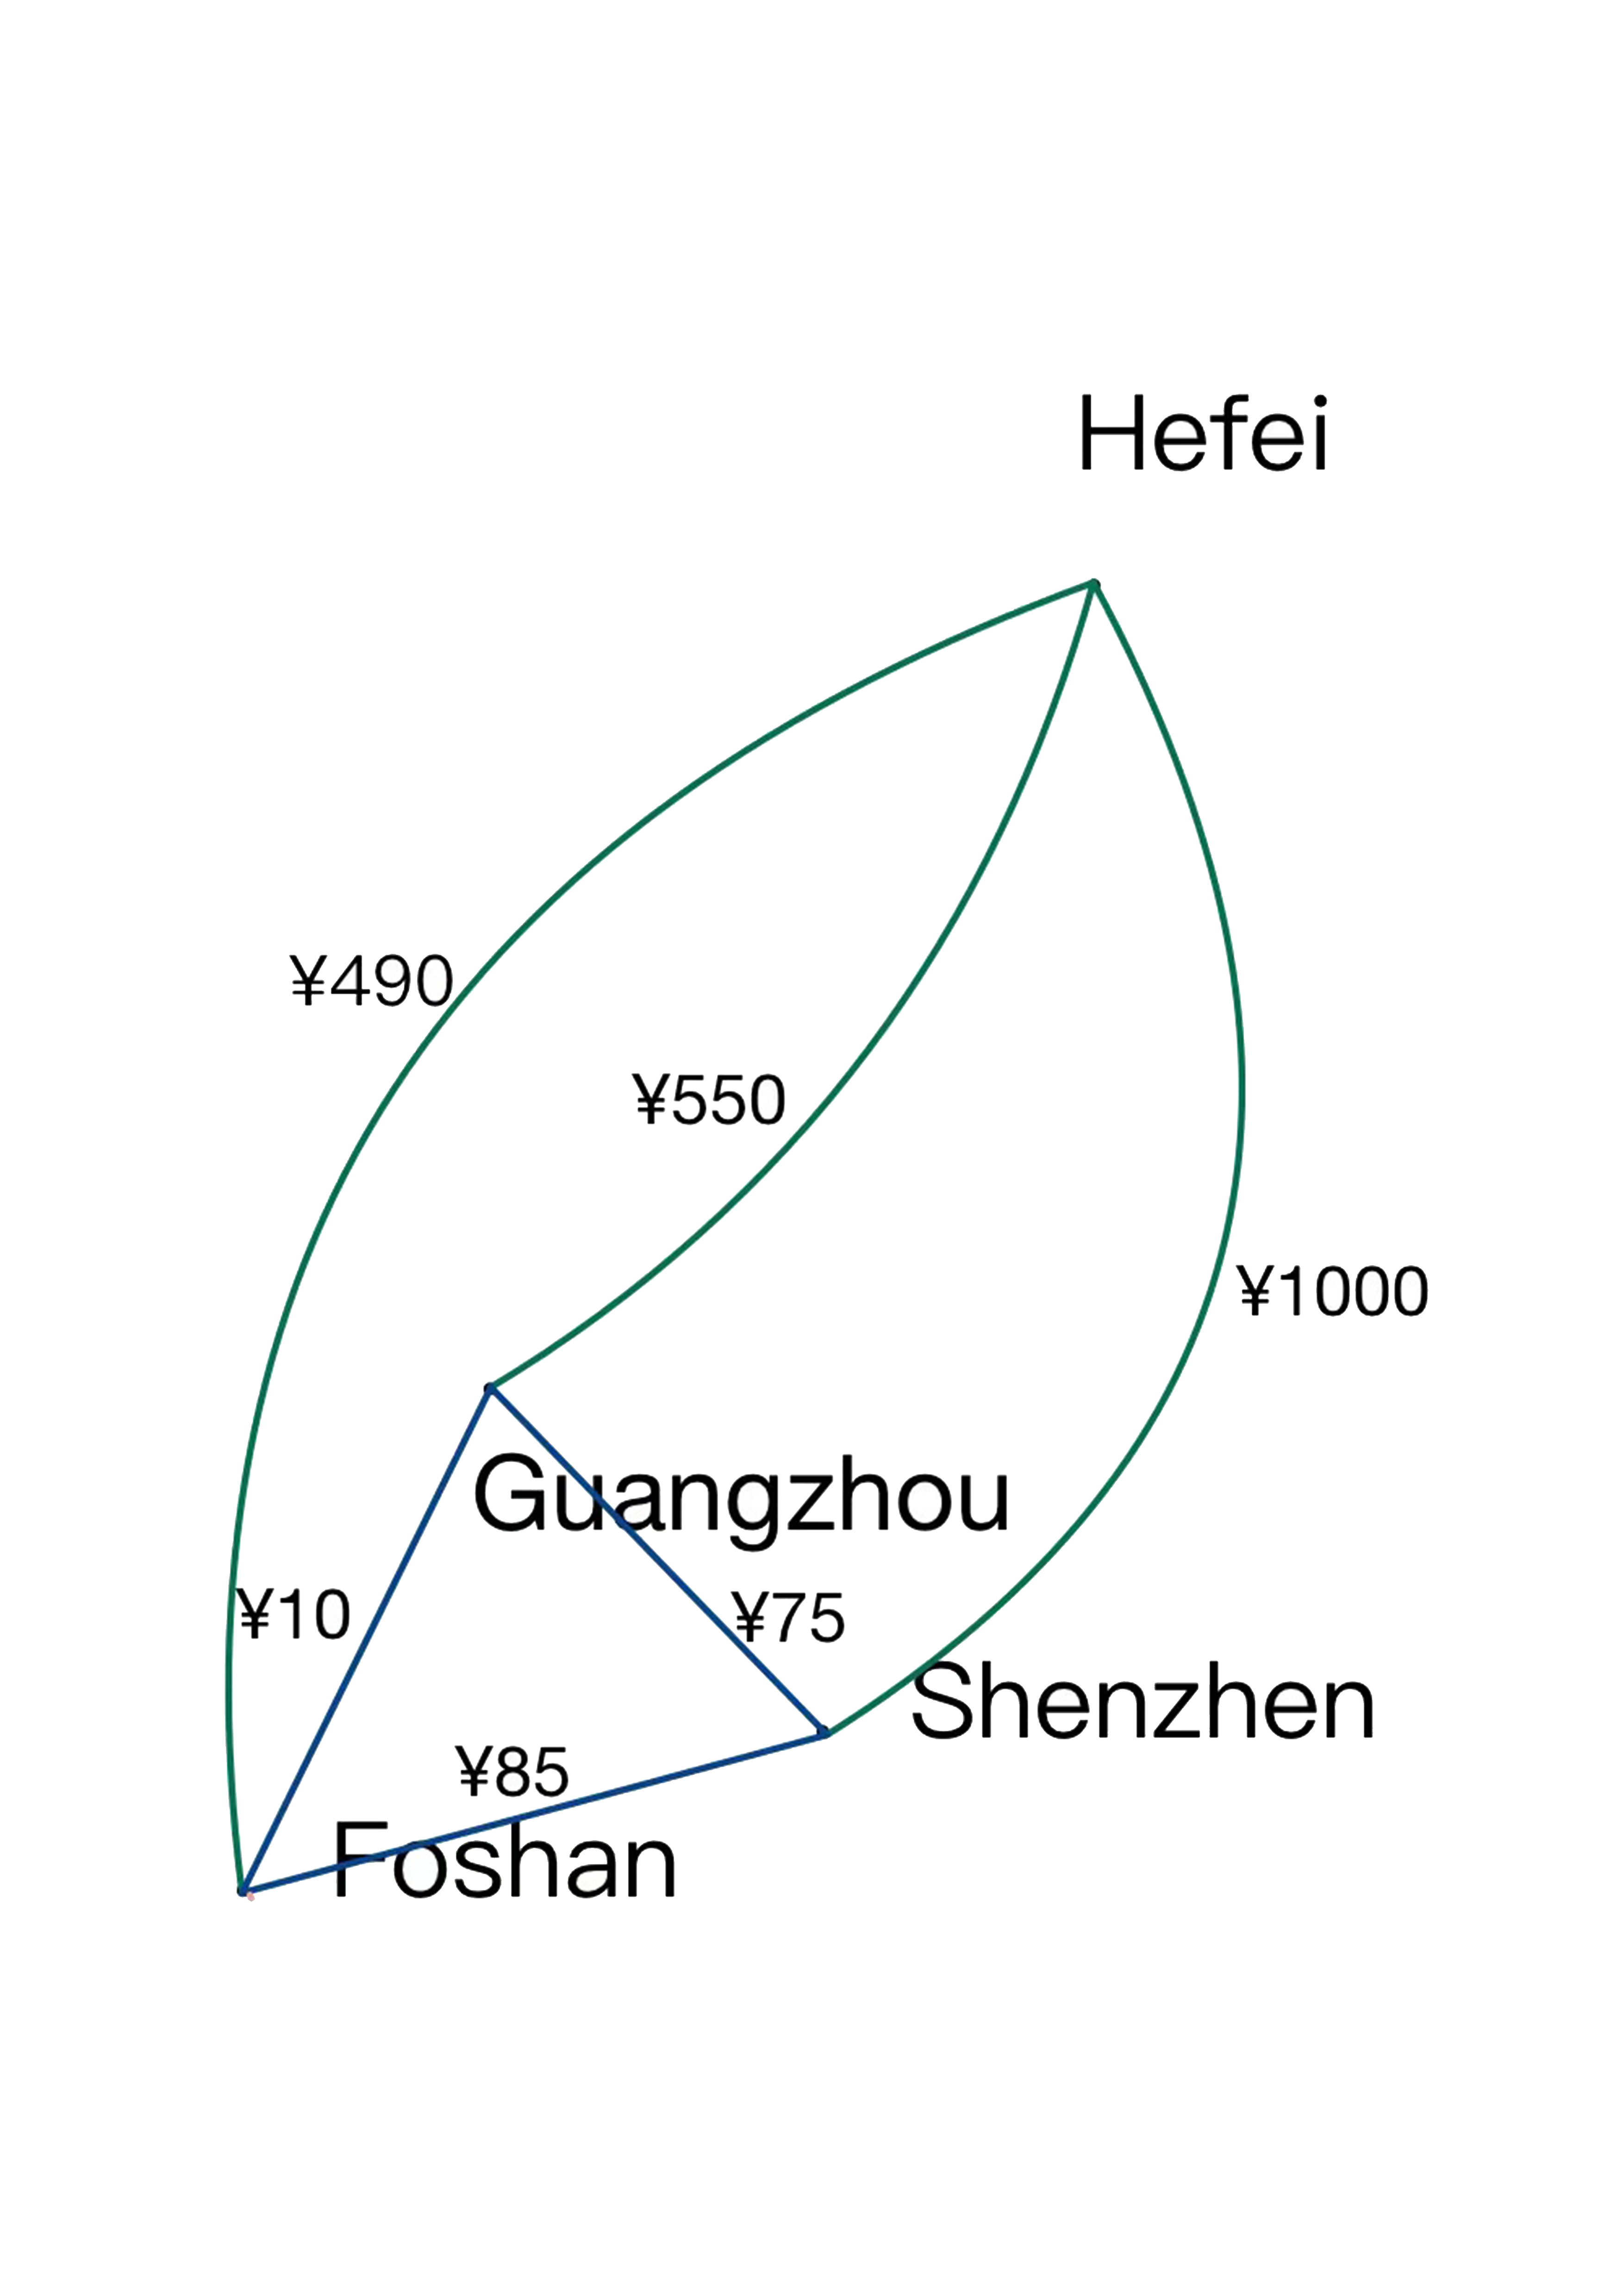
\includegraphics[width=0.85\textwidth]{pic/1.png}
    \caption{Ticket Prices}%
    \label{fig:your_image1}
  \end{subfigure}
  \hfill % Add space between images
  \begin{subfigure}{0.3\textwidth}
    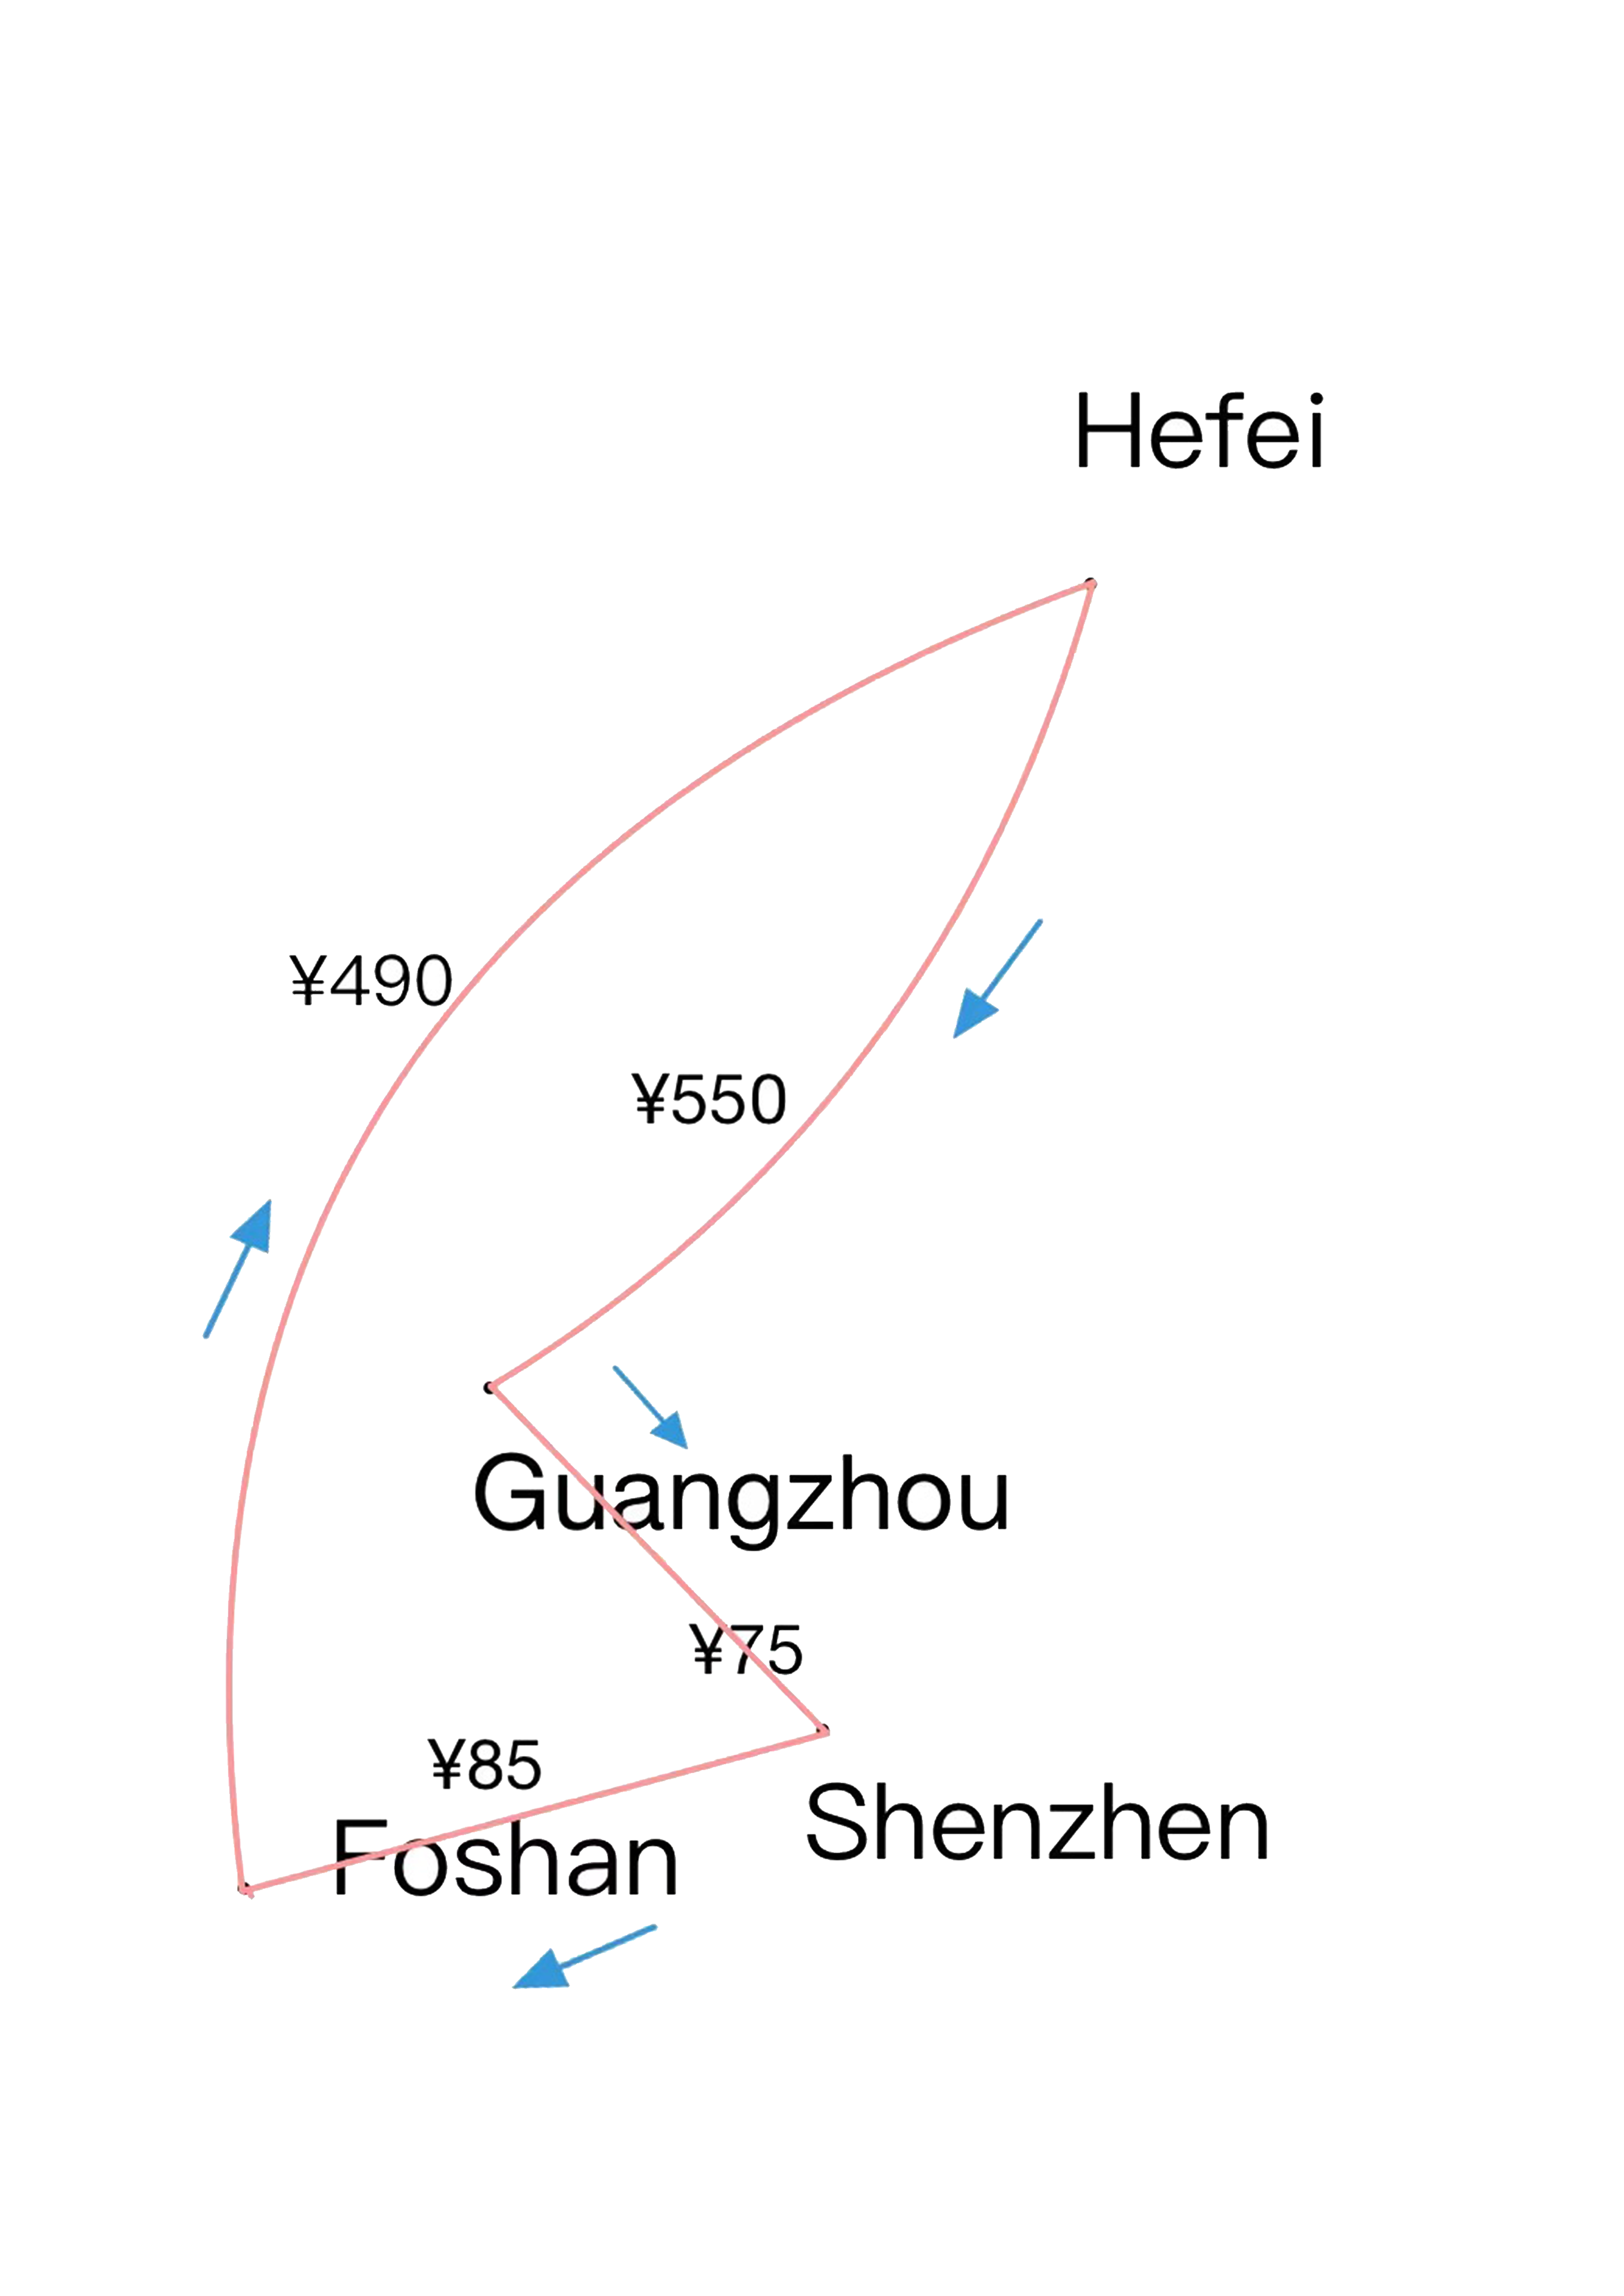
\includegraphics[width=0.85\textwidth]{pic/2.png}
    \caption{Optimal Choice}%
    \label{fig:your_image2}
  \end{subfigure}%
  \hfill % Add space between images
  \begin{subfigure}{0.3\textwidth}
    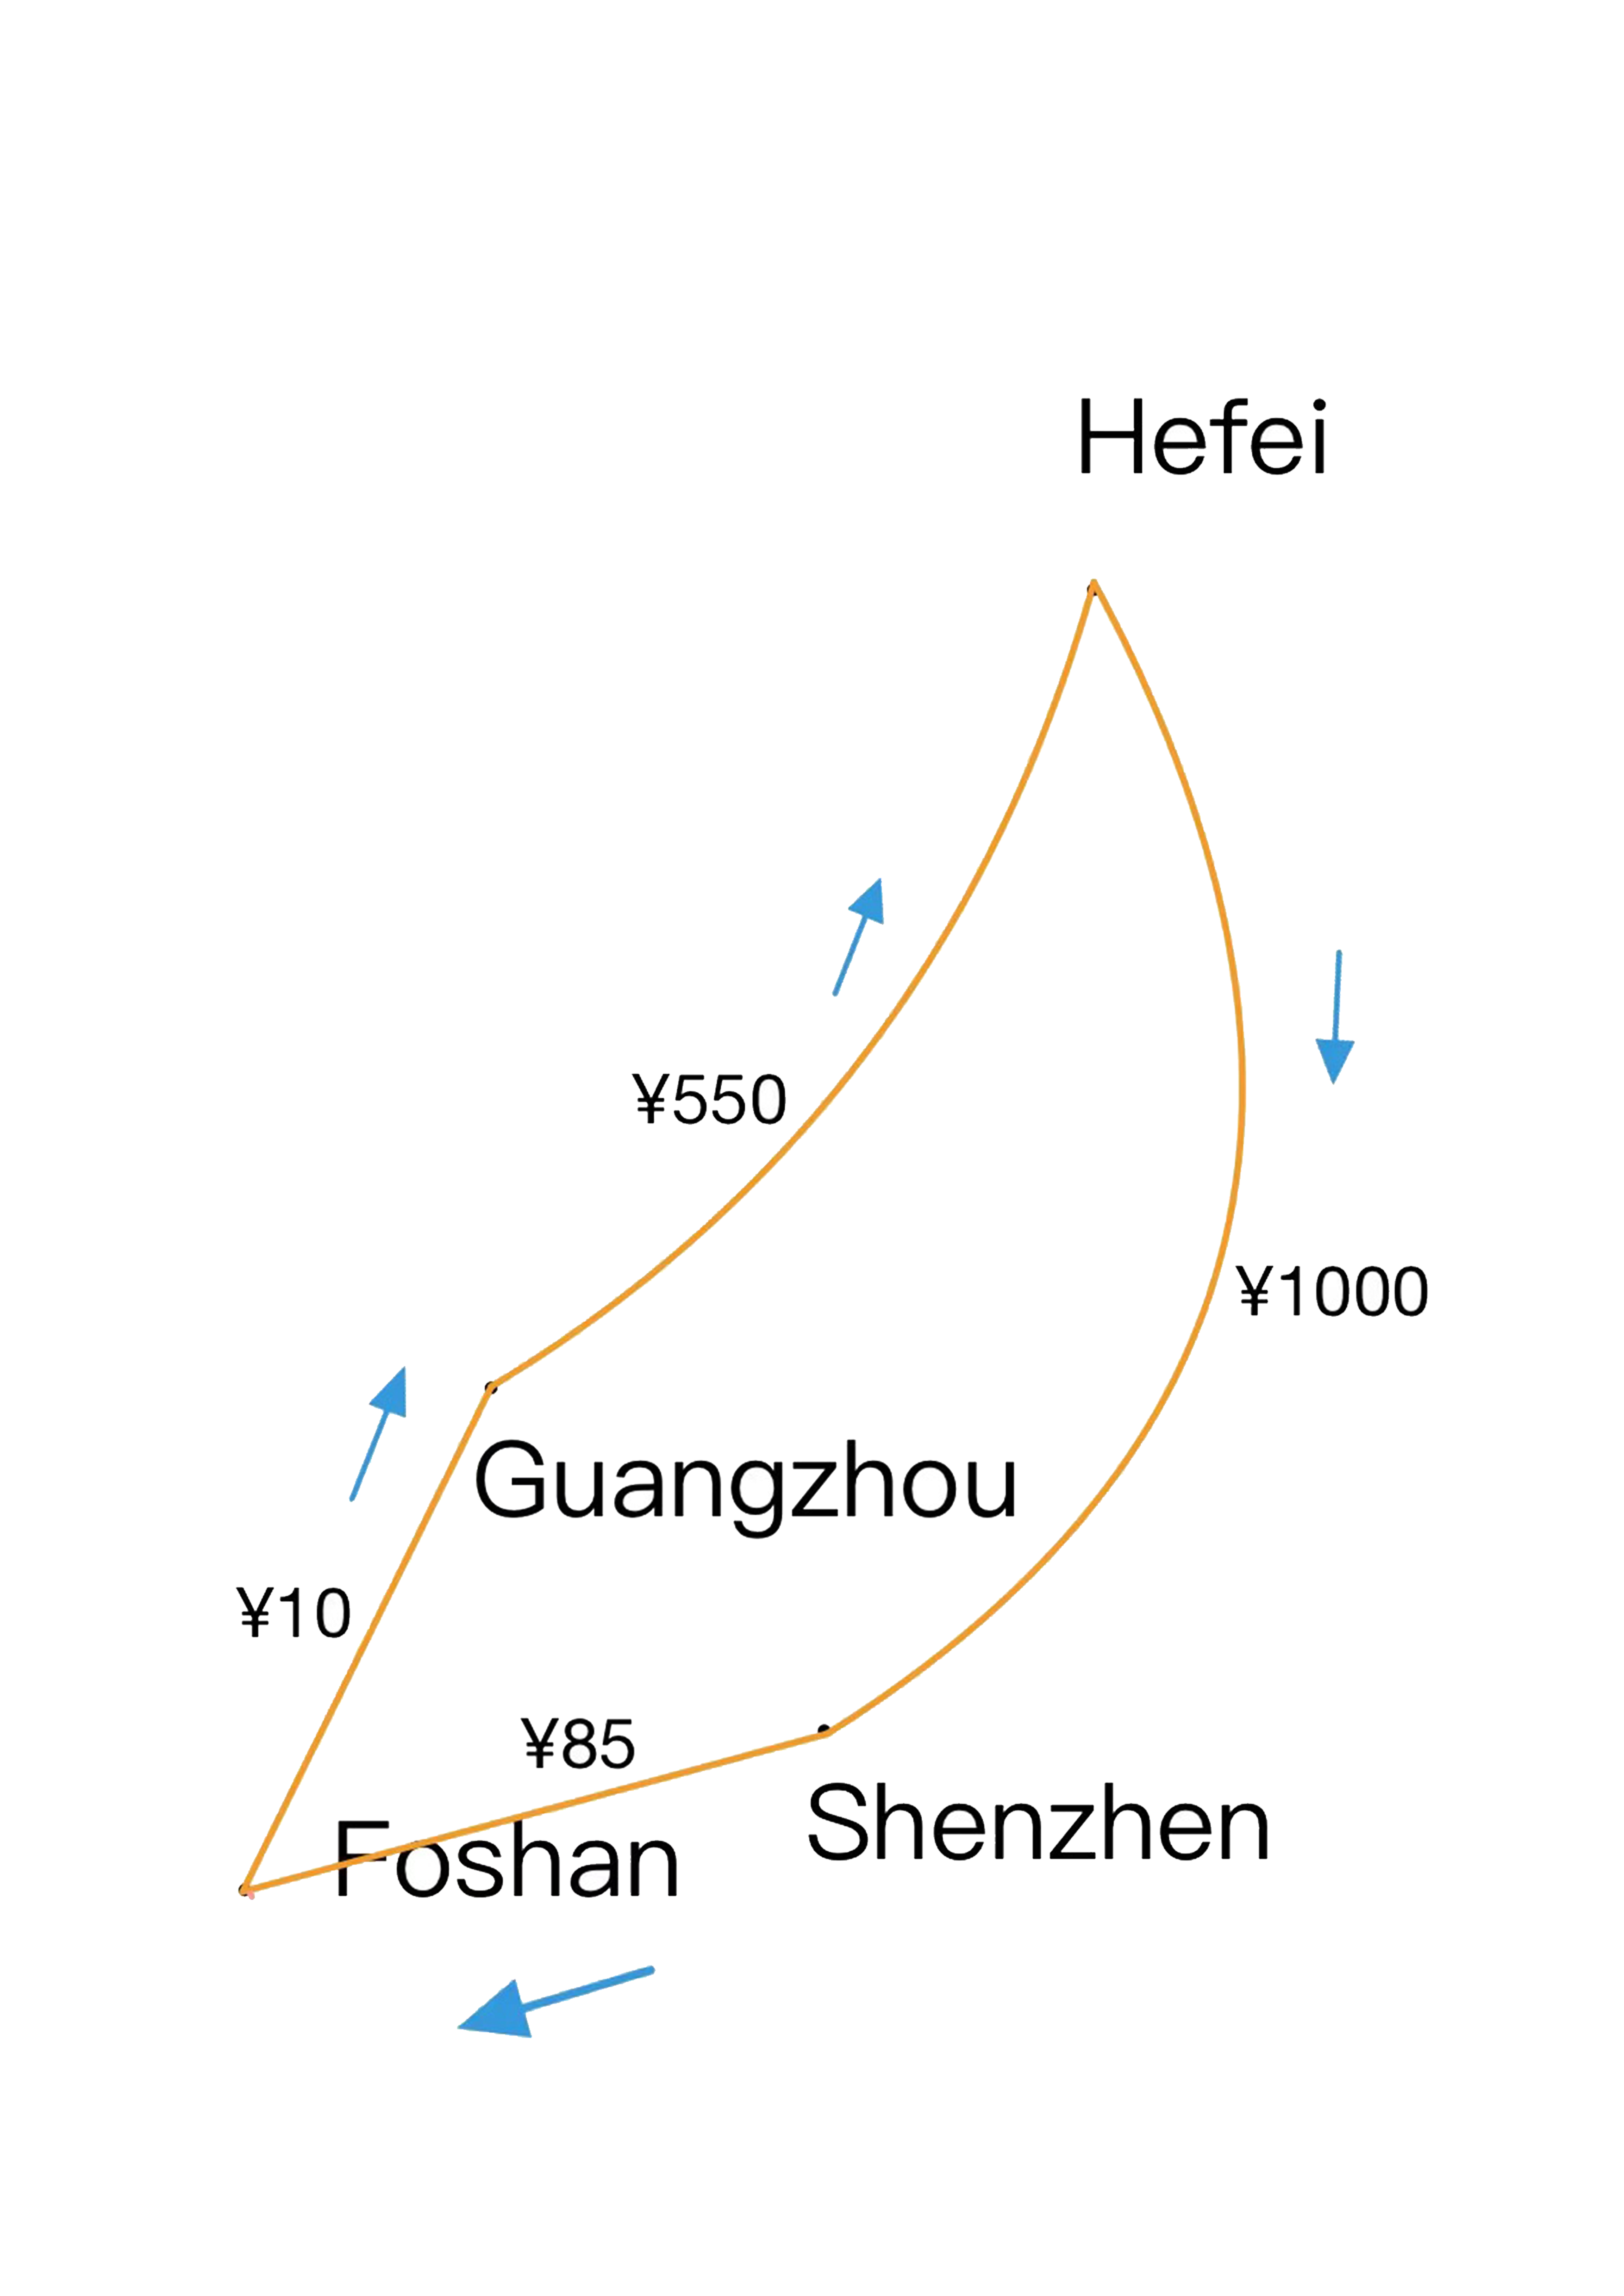
\includegraphics[width=0.85\textwidth]{pic/3.png}
    \caption{Choice With Higher Price}%
    \label{fig:your_image3}
  \end{subfigure}%
\end{figure}
\section{MIP Model}
Let $G_1(V_1, E_1)$ and $G_2(V_2, E_2)$ be two given graphs, each with their
respective vertex and edge sets. Define a positive edge weight function $w :
  E_1 \cup E_2 \rightarrow \mathbb{R}^+$. We construct a new graph $G(V, E)$,
where $V = V_1 \cup V_2$ and $E = E_1 \cup E_2$. The objective is to find a
Hamiltonian cycle in $G$ that minimizes the objective function. In order to
achieve this, we introduce binary variables $x_{ij}^k$ for edge selection from
either $G_1$ or $G_2$.

Formally, let $x_{ij}^k \in \{0, 1\}$ be a binary variable such that:

\begin{equation*}
  x_{ij}^k =
  \begin{cases}
    1, & \text{if edge } (i, j) \text{ from graph } G_k \text{ is selected,} \\
    0, & \text{otherwise.}
  \end{cases}
\end{equation*}

The goal is to determine the values of $x_{ij}^k$ that lead to a Hamiltonian
cycle with the minimum objective function value in the graph $G$. It can be
written as:
\begin{equation*}
  \text{minimize} \, f = \sum_{k=1}^{2} \sum_{(i,j) \in E_k} w_{ij}^k x_{ij}^k
\end{equation*}

Subject to the following \textbf{constraints}:

\begin{enumerate}
  \item Each vertex has a total degree of 2, with one incoming edge (in-degree) and one
        outgoing edge (out-degree) from either graph $G_1$ or $G_2$.

        \begin{equation*}
          \sum_{k=1}^{2} \sum_{j \in V} x_{ij}^k = 2, \quad \forall i \in V
        \end{equation*}
  \item No subtours are allowed (subtour elimination constraint):

        \begin{equation}
          \sum_{(i,j) \in S \times (V \setminus S)} x_{ij}^k \geq 2, \quad \forall S \subset V, S \neq \emptyset, S \neq V, k \in \{1, 2\}
        \end{equation}

        Here, $S$ is a subset of $V$, and $(V \setminus S)$ is the complement of $S$ in
        $V$. $(1)$ ensures that there are no smaller cycles within the Hamiltonian
        cycle.
  \item The number of edges selected from $G_1$ and $G_2$ are no more than $N_1$ and
        $N_2$ respectively.

        \begin{equation*}
          \sum_{(i,j) \in E_1} x_{ij}^1 \leq N_1 \quad \text{and} \quad \sum_{(i,j) \in E_2} x_{ij}^2 \leq N_2,  \quad \forall i,j \in V
        \end{equation*}
\end{enumerate}

\subsection*{Variables and Parameters}
In our case, the variables and parameters are defined as follows:
\begin{itemize}
  \item $G_1(V_1, E_1)$ and $G_2(V_2, E_2)$ store the information of airplane's and train's transportation modes.
  \item The vertices $V_1$ and $V_2$ in each graph represent cities in different
        countries.
  \item $k$ is an index representing the transportation mode in the given graphs. Specifically, $k = 1$ corresponds to the airplane transportation mode in graph $G_1$, and $k = 2$ corresponds to the train transportation mode in graph $G_2$.
  \item If there is an edge between the vertices, it indicates that travel between the
        cities is accessible using either mode of transportation. We can represent an
        edge between vertex $i$ and $j$ as $(i, j) \in E_k$, where $k \in \{1, 2\}$.
  \item The edges store $cost$ and $time$, which represent the one-way ticket price and
        travel time, respectively. So the weight function $w$ is defined as:
        \begin{equation*}
          w_{ij}^k = \alpha \cdot \text{cost}_{ij}^k + \beta \cdot \text{time}_{ij}^k, \quad where \quad \alpha + \beta = 1
        \end{equation*}

        where $\alpha$ and $\beta$ are the weights of the cost and time attributes
        respectively.

\end{itemize}
Therefore, our objective function can be further written as:

\begin{equation*}
  \text{minimize}\, f = \sum_{k=1}^{2} \sum_{(i,j) \in E_k} (\alpha \cdot \text{cost}_{ij}^k + \beta \cdot \text{time}_{ij}^k) x_{ij}^k
\end{equation*}

\section{Computational Results}
\begin{table}[!ht]
  \centering
  \begin{tabular}{llrrr}
    \toprule
    Segment                          & Transportation Mode & Cost (¥) & Time (hours) \\
    \midrule
    London $\rightarrow$  Paris      & Airplane            & 459.0    & 1.05         \\
    Paris $\rightarrow$  Budapest    & Airplane            & 1171.0   & 0.83         \\
    Budapest $\rightarrow$  Vienna   & Airplane            & 794.0    & 0.83         \\
    Vienna $\rightarrow$  Rome       & Airplane            & 344.0    & 1.45         \\
    Rome $\rightarrow$  Barcelona    & Airplane            & 634.0    & 2.0          \\
    Barcelona $\rightarrow$  Zurich  & Airplane            & 760.0    & 1.92         \\
    Zurich $\rightarrow$  Copenhagen & Airplane            & 855.0    & 1.75         \\
    Copenhagen $\rightarrow$  Berlin & Airplane            & 317.0    & 1.0          \\
    Berlin $\rightarrow$  Amsterdam  & Airplane            & 967.0    & 1.4          \\
    Amsterdam $\rightarrow$  London  & Airplane            & 940.0    & 1.1          \\
    \midrule
    Total                            &                     & 7241.0   & 13.0         \\
    \bottomrule
  \end{tabular}
  \caption{$\alpha=0, \beta=1$}%
  \label{tab:city-travel}
\end{table}
Different weight functions result in different
consequences\cite{lamport1994latex}.
\subsection*{Sensitive Analysis}
\section{Conclusion}
\section{Appendix}
\section{References}
\printbibliography[heading=none]

\end{document}